\documentclass[a4paper,11pt]{article}

\usepackage[french,italian]{babel}
\usepackage[T1]{fontenc}
\usepackage[utf8]{inputenc}
\frenchspacing 
\title{Analisi dell'efficienza di un'algoritmo mergesort ibrido}
\author{Luca Seggiani}
\date{21 Marzo 2024}

\usepackage{graphicx}
\usepackage{listings}
\usepackage{xcolor}

\definecolor{codegreen}{rgb}{0,0.6,0}
\definecolor{codegray}{rgb}{0.5,0.5,0.5}
\definecolor{codepurple}{rgb}{0.58,0,0.82}
\definecolor{backcolour}{rgb}{0.95,0.95,0.92}

\lstdefinestyle{code-style}{
    backgroundcolor=\color{backcolour},   
    commentstyle=\color{codegreen},
    keywordstyle=\color{magenta},
    numberstyle=\tiny\color{codegray},
    stringstyle=\color{codepurple},
    basicstyle=\ttfamily\footnotesize,
    breakatwhitespace=false,         
    breaklines=true,                 
    captionpos=b,                    
    keepspaces=true,                 
    numbers=left,                    
    numbersep=5pt,                  
    showspaces=false,                
    showstringspaces=false,
    showtabs=false,                  
    tabsize=2
}

\lstset{style=code-style}

\begin{document}
\maketitle
\section{Implementazione}
Si implementa un'algoritmo di ordinamento di vettori basato su un'approccio ibrido tra mergesort ed insertion sort. L'implementazione del mergesort è ricorsiva, ed è previsto l'utilizzo di un'array d'appoggio per
la ricombinazione degli array. Al passo ricorsivo, se la dimensione della sottoarray è rilevata come inferiore ad un certo valore \textit{threshold}, si esegue un'insertion sort su quella specifica sottoarray. L'implementazione
del mergesort è la seguente:
\begin{lstlisting}[language=C++]
void merge(int arr[], int beg, int mid, int end) {
    int iS = beg;
    int iD = mid;

    vector<int> temp;

    while(true) {
        if(arr[iS] <= arr[iD]) {
            temp.push_back(arr[iS++]);
            if(iS >= mid) {
                while(iD < end) temp.push_back(arr[iD++]);
                break;
            }
        } else {
            temp.push_back(arr[iD++]);
            if(iD >= end) {
                while(iS < mid) temp.push_back(arr[iS++]);
                break;
            }
        }
    }

    for(int i = 0; i < temp.size(); i++) {
        arr[i + beg] = temp[i];
    }

}

void mergeSort(int vett[], int beg, int end) {
    if(beg + 1 < end) {
        int mid = (beg + end) / 2;
        mergeSort(vett, beg, mid);
        mergeSort(vett, mid, end);
        merge(vett, beg, mid, end);
    }
}
\end{lstlisting}
dove la funzione merge effettua la ricombinazione di due sottoarray all'interno dello stesso array, attraverso due indici (che partono dalla posizione iniziale e media) e un vettore ausiliario STL.
Si implementa poi l'insertion sort:
\begin{lstlisting}[language=C++]
void insertion_sort(int vett[], int beg, int end) {
  int current = 0, p = 0;
  for(int i = beg + 1; i < end; i++) {
    current = vett[i];
    p = i - 1;

    while(p >= 0 && vett[p] > current) {
      vett[p + 1] = vett[p];
      p--;
    }
    vett[p + 1] = current;
  }
}

void print_vett(int vett[], int size) {
  for(int i = 0; i < size; i++) {
    cout << vett[i] << "\t";
  }
  cout << endl;
}
\end{lstlisting}
e se ne implementa la chiamata nel caso in cui la dimensione d'istanza rilevata nel passo ricorsivo del mergesort sia minore ad un certo valore \textit{threshold}:
\begin{lstlisting}[language=C++]
void mergeSort(int vett[], int beg, int end) {
    if(beg + 1 < end) {
        if(end - beg < threshold) {
          insertion_sort(vett, beg, end);
          return;
        }
        int mid = (beg + end) / 2;
        mergeSort(vett, beg, mid);
        mergeSort(vett, mid, end);
        merge(vett, beg, mid, end);
    }
}
\end{lstlisting}
\section{Analisi}
Il codice sopra riportato è compilato in un eseguibile che prende 3 argomenti: la dimensione d'istanza, il valore \textit{threshold}, e un valore \textit{seme} usato per la generazione casuale
di array disordinati della dimensione d'istanza richiesta. Attraverso un'utility scritta in Python si chiama il programma per un numero determinato di istanze (per questa analisi è stato scelto 15),
calcolandone il tempo di esecuzione medio attraverso il comando time della shell bash. I dati risultanti vengono compilati in un grafico che ha sull'asse x la dimensione d'istanza e sull'asse y il tempo
medio dell'algoritmo, e dove i diversi valori threshold corrispondono a colori a tonalità crescente:
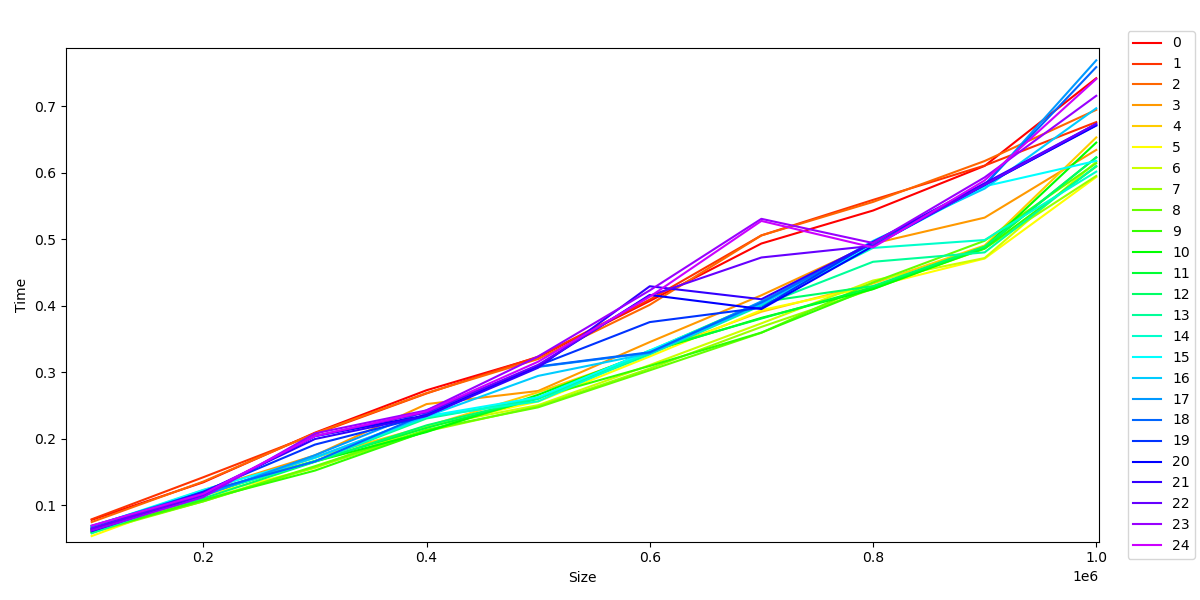
\includegraphics[scale = 0.5]{Figure_1.png}
Dal grafico si nota che l'efficienza maggiore in termini di tempo è raggiunta con un threshold compreso fra 6 e 10, e che comunque un valore superiore a 3 (dove si può immaginare inizi ad avere effetto l'azione dell'insertion sort)
è quasi sempre meglio del non avere nessuna ottimizzazione.
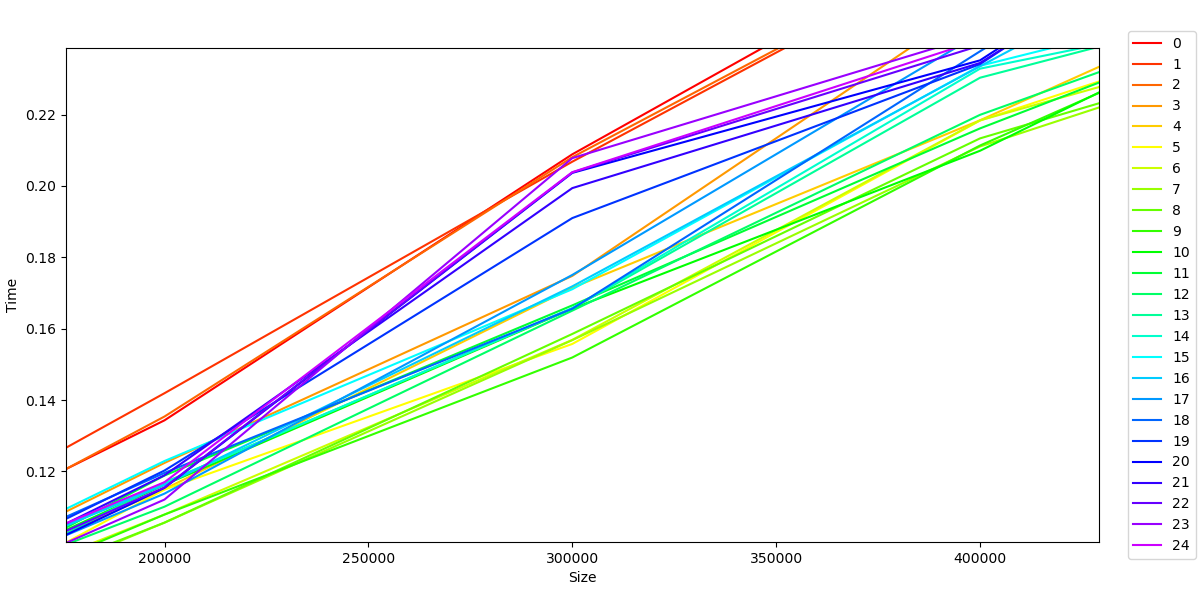
\includegraphics[scale = 0.23]{Figure_2.png}
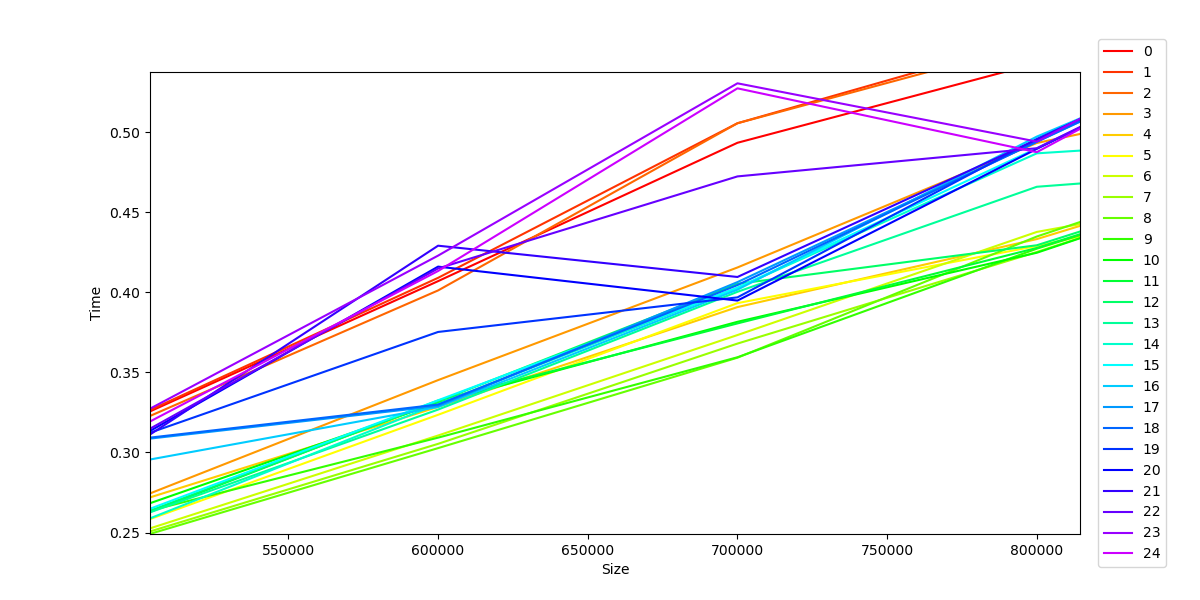
\includegraphics[scale = 0.23]{Figure_3.png}
\end{document}
